\documentclass{beamer}
\usetheme{Madrid}
\usecolortheme{beaver}
\usepackage{graphicx}
\graphicspath{ {pics} }

%Information to be included in the title page:
\title{Real Numbers}
\author{Nithin}
\institute{Maveric Systems}
\date{\today}

\begin{document}
\frame{\titlepage}

\begin{frame}{Integers}
    \begin{itemize}
        \item The set of integers is denoted by \(\mathbb{Z}\).
        \item Integers include:
        \[
          \ldots, -3, -2, -1, 0, 1, 2, 3, \ldots
        \]
        \item Formally, \(\mathbb{Z} = \{\dots, -2, -1, 0, 1, 2, \dots\}\).
        \item Common properties:
        \begin{itemize}
            \item \(\mathbb{Z}\) is infinite and unbounded in both the negative and positive directions.
            \item Closed under addition, subtraction, and multiplication:
                \[
                  \forall a, b \in \mathbb{Z}, \quad
                  a \pm b \in \mathbb{Z}, \quad
                  a \cdot b \in \mathbb{Z}.
                \]
        \end{itemize}
        \item The quotient of any two integers is not necessarily an integer. So we need to extend arithmetic to \textbf{rational numbers}
    \end{itemize}
\end{frame}

% Slide: Rational Numbers
\begin{frame}{Rational Numbers}
    \begin{itemize}
        \item The set of rational numbers is denoted by \(\mathbb{Q}\).
        \item Definition:
        \[
          \mathbb{Q} = \left\{ \frac{p}{q} \,\middle|\,
            p \in \mathbb{Z}, \; q \in \mathbb{Z}, \; q \neq 0
          \right\}.
        \]
        \item Every integer is also a rational number (e.g., \(5 = \frac{5}{1}\)).
        \item Examples:
        \[
          \frac{1}{2}, \quad -\frac{3}{4}, \quad 0, \quad 7, \quad \frac{11}{5}, \ldots
        \]
        \item Properties:
        \begin{itemize}
            \item Closed under addition, subtraction, multiplication, and division (except division by zero).
            \item Densely packed on the number line: between any two rationals, there is another rational.
        \end{itemize}
    \end{itemize}
\end{frame}

\begin{frame}
    \frametitle{Interesting Facts}
    \begin{itemize} 
        \item Why division by zero is prohibited ?
        \begin{itemize}
            \item Division is inverse of multiplication in the sense  
            \[  
            \frac{m}{n} \cdot n = m
            \]
        \item if \( n=0 \) and \( m = 1\), we get \(\frac{1}{0} \cdot 0 = 1\) which is nonsensical as any number multiplied by zero is zero
        \end{itemize}
        \item Rational numbers suffice for all actual physical measurements like weight, height and length
        \item But Geometry, Algebra and Calculus force us to consider \textbf{real numbers}
    \end{itemize}

\end{frame}

\begin{frame}
    \frametitle{A Real Number Line}
    \begin{figure}[h]    
        \begin{minipage}[b]{0.8\textwidth}
        \centering
        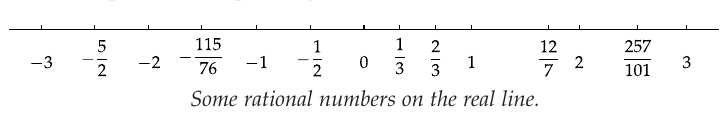
\includegraphics[scale=0.35]{real-line.png}
    \end{minipage}
\end{figure}
\begin{itemize}
    \item if \( n\) is a positive integer then \( \frac{1}{n}\) is to the right of 0 by the length obtained by dividing the segment from \( 1 to 0\) in to \( n \) segments of equal length
\end{itemize}

\end{frame}

\begin{frame}
    \frametitle{Is every Real Number a Rational}
    \begin{figure}[h]    
        \begin{minipage}[b]{0.8\textwidth}
        \centering
        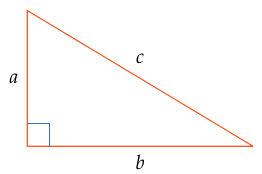
\includegraphics[scale=0.35]{irrational-geometry.png}
        \end{minipage}
    \end{figure}
    \begin{itemize}
        \item \( c^{2} = a^{2} + b^{2} \). If \( a = 1, b = 1\) then \(c^{2} = 2 \). Then what rational number is \( c \)
        \item By trial and error let assume \( c = \left( \frac{99}{70} \right)^{2}  = \frac{9801}{4900}\) where the numerator just misses twice the denominator by 1  
    \end{itemize} 
\end{frame}



\end{document}